% !TeX TS-program = xelatex
% This is SJTUBeamermin v1.0
% For more detailed desciption, see
% https://github.com/LogCreative/SJTUBeamermin/blob/main/doc/sjtubeamermintheme.pdf
%
\documentclass[
    % draft,                             % 草稿模式
    aspectratio=169,                   % 使用 16:9 比例
]{beamer}
\mode<presentation>
\usetheme[
    navigation=subsections,            % 使用子章节进度显示
     lang=en,                           % 使用英文
    % cjk=true,                          % 使用CJK而不是ctex
    color=blue,                         % 使用红色主题
    % pattern=all,                        % 使用全图案装饰
    % gbt=bibtex,                        % 使用 gbt (使用 bibtex 编译)
]{sjtubeamermin}
% \usecolortheme[]{beaver}                 % 使用其他颜色主题
% \addbibresource{ref.bib}               % gbt!=bibtex

\usepackage{amsmath,amsthm}
\usepackage{bm}
\usepackage{tikz-cd}
\usepackage{tikz}
\usetikzlibrary{trees}
\usepackage{empheq}
\usepackage{tabularx}
\usepackage{pifont}
\usepackage{multicol}
\usepackage[linesnumbered,ruled]{algorithm2e}
\usepackage{hyperref}
\usepackage{amsfonts}
\usepackage{tasks}
\usepackage{fontspec}
\usepackage{mdframed} % Add easy frames to paragraphs
\usepackage{color,soul}
\usepackage{xparse} % Add support for \NewDocumentEnvironment

\usepackage[customcolors]{hf-tikz}
\tikzset{style green/.style={
    set fill color=green!50!lime!60,
    set border color=white,
  },
  style cyan/.style={
    set fill color=cyan!90!blue!60,
  },
  style orange/.style={
    set fill color=orange!80!red!60,
  },
  hor/.style={
    above left offset={-0.31,0.31},
    below right offset={0.31,-0.2},
    #1
  },
  ver/.style={
    above left offset={-0.1,0.3},
    below right offset={0.15,-0.15},
    #1
  }
}

\renewcommand{\Bbb}{\mathbb}
\newcommand{\Z}{\mathbb{Z}}
\newcommand{\GR}{\mathbb{GR}}
\newcommand{\F}{\mathbb{F}}
\newcommand{\R}{\mathbb{R}}
\newcommand{\Fns}{\mathbb{F}_{2^n}^*}
\newcommand{\Fn}{\mathbb{F}_{2^n}}
\newcommand{\Fks}{\mathbb{F}_{2^k}^*}
\newcommand{\Fk}{\mathbb{F}_{2^k}}
\newcommand{\df}{\delta_F}
\newcommand{\tr}{\operatorname{tr}_1^k}
\newcommand{\gtr}{\operatorname{T}}
\newcommand{\Bn}{\mathcal{B}_n}
\newcommand{\teich}{\textit{Teichm$\ddot{u}$ller sets}}
% \newtheorem*{definition}{Definition}
\newtheorem{thm}{Theorem}
\newtheorem{lem}[thm]{Lemma}
\newtheorem{proposition}{Proposition}
\definecolor{graylight}{cmyk}{.30,0,0,.67} % define color using xcolor syntax
\setbeamertemplate{itemize items}[default]

% modify the footnote symbol 
% \makeatother
% \renewcommand{\thefootnote}{\ifcase\value{footnote}\or\dagger\or(\#\#)\or(\#\#\#)\or(\#\#\#\#)\or(\#\#\#\#\#)\fi}
% \makeatletter



\newmdenv[ % Define mdframe settings and store as leftrule
  linecolor=red,
  topline=false,
  bottomline=false,
  rightline=false,
  skipabove=\topsep,
  skipbelow=\topsep
]{leftrule}

% \NewDocumentEnvironment{example}{O{\textbf{Example:}}} % Define example environment
% {\begin{leftrule}\noindent\textcolor{blue}{#1}\par}
% {\end{leftrule}}
\setbeamertemplate{footline}[frame number]

\NewDocumentEnvironment{question}{O{\textbf{Something:}}} % Define something environment
{\begin{leftrule}\noindent\textcolor{graylight}{#1}\par}
{\end{leftrule}}

\NewDocumentEnvironment{remark}{O{\textbf{Remark:}}} % Define remark environment
{\begin{leftrule}\noindent\textcolor{blue}{#1}\par}
{\end{leftrule}}

\begin{document}
    \institute[School of Electronic Information and Electrical Engineering]{电子信息与电气工程学院}   % 组织
    % \logo{
    %     
\includegraphics{support/cnlogored.pdf}  % 重定义 logo
    % }
    \titlegraphic{                         % 标题图像
        \begin{stampbox}[white]
            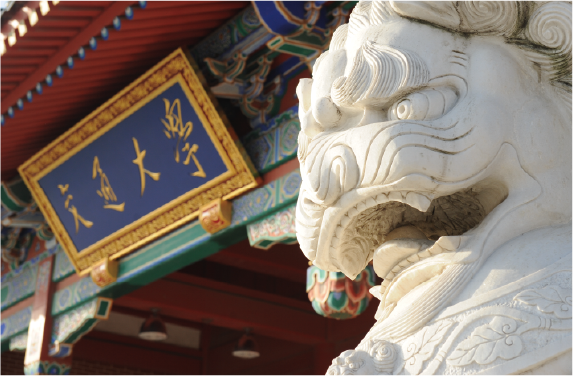
\includegraphics[width=0.3\textwidth]{support/head.png}
        \end{stampbox}
    }
    \title{Higher order nonlinearity of bent functions}  % 标题
 %   \subtitle{SJTUBeamer \fbox{\textsc{min}} Template}         % 副标题
    \author{Zhaole Li}                  % 作者
    \date{\textcolor{red}{2022/11/1}}                          % 日期
    \maketitle                             % 创建标题页


\AtBeginSection[]{
   \begin{frame}
       % \tableofcontents[currentsection]           % 传统节目录             
       \sectionpage                   % 节页
   \end{frame}
}

% 使用小节目录
%\AtBeginSubsection[]{                  % 在每小节开始
 %   \begin{frame}
        % \tableofcontents[currentsection,currentsubsection]             % 传统小节目录             
  %      \subsectionpage                % 小节页
 %   \end{frame}
%}

% \section{Introduction}
%\subsection{第 1 小节}
    \begin{frame}
        \frametitle{Boolean functions}
        \begin{itemize}
            \item We call $ n $-variable Boolean functions or Boolean functions in dimension $ n $ the functions from 
            the $ n $-dimensional vector space $ \F_2^n $ over $ \F_2 $ to $ \F_2 $. 

            \item Their set is denoted by $ \Bn $, where $ n $ is the number of variables of Boolean functions.
            
            \item Given a basis, the field $ \Fn $ can be identified with the vector space $ \F_2^n $. 
            Thus the input of Boolean functions will also be considered in the field $ \Fn $.
        \end{itemize}

    \end{frame}

    \begin{frame}
        \frametitle{Representation of Boolean functions}
    
        \begin{itemize}
            \item Truth Table:
            \scalebox{0.7}{
            $\begin{array}{cccc}
                \hline\hline 
                x_1 & x_2 & x_3 & f(x) \\
                \hline 
                0 & 0 & 0  & 0 \\
                0 & 0 & 1  & 1 \\
                0 & 1 & 0  & 0 \\
                0 & 1 & 1  & 0 \\
                1 & 0 & 0  & 0 \\
                1 & 0 & 1  & 1 \\
                1 & 1 & 0  & 0 \\
                1 & 1 & 1  & 1 \\
                \hline\hline
            \end{array}$ corresponding to $ 3 $-variable Boolean function $ f(x_1,x_2,x_3)=x_1x_2x_3+x_2x_3+x_3 $
            in ANF.
            }
            \item Algebraic Normal Form: 
            \[f(x_1,\dots,x_n) = \bigoplus_{I\subseteq\{1,\dots,n\}}a_I\left(\prod_{i\in I}x_i \right).\]
            \item Univariate Representation: 
            \[f(x) = \sum_{i=0}^{2^n-1}\delta_ix^i.\]
        \end{itemize}
    
    \end{frame}

    \begin{frame}
        \frametitle{Trace functions}
    
        \begin{definition}
            Let $ F = \F_{2^m} $, $ K = \F_{2^n} $ where $ m\mid n $. We may view $ F $ as a subfield of $ K $. 
            If $ \alpha $ is an element of $ K $, its trace relative to the subfield $ F $ is defined as follows: 
            \[\operatorname{tr}_F^K(\alpha)=\alpha+\alpha^{2^m}+\alpha^{2^{2m}}+\cdots+\alpha^{2^{\frac{n}{m}-1}m}.\]
        \end{definition}
        When no confusion is likely to arise, we will simply write the trace function as $ \operatorname{tr}_m^n(\alpha) $.
        \begin{remark}
            Trace function $ \operatorname{tr}_m^n $ is a $ F $-linear tranformation from $ K $ onto $ F $ and is balanced.
        \end{remark}
    
    \end{frame}
    \begin{frame}
        \frametitle{Walsh transform and Hamming distance}
    
        \begin{definition}
            We call the Walsh transform of a Boolean function $f$ the Fourier transform of 
            the function $ (-1)^{f(x)} $, and we denote it by $ W_f $: 
            \[W_f(u) = \sum_{x\in\F_{2}^n}(-1)^{f(x)+u\cdot x}.\]
        \end{definition}
        \begin{definition}
            The Hamming distance between $f,g\in\Bn$ is given by \[ d_H(f,g) = |\left\{x\in\F_2^n\middle|f(x)\ne g(x)\right\}|.\]
        \end{definition}
    \end{frame}
    \begin{frame}
        \frametitle{The $ r $th-order nonlinearity for Boolean functions}
        
        \begin{definition}[Algebraic Degree]
            The degree of Boolean function $ f $ is denoted by $ deg(f) $ and is called the algebraic degree of the function: 
            $ deg(f) = \max\{|I|: a_I \ne 0\} $, where $ |I| $ denotes the size of $ I $.
        \end{definition}

        % The $ r $th-order nonlinearity is an important parameter of a Boolean function $ f $:
        \begin{example}
            $ f=x_1x_2x_3+x_2x_3+x_3 $ is a $3$-variable Boolean function over $ \F_2^n $ with $ deg(f)=3 $.
            The Hamming distance between $ f $ and $ g=x_3 $ is $ 1 $.
        \end{example}
        \begin{remark}
            The Hamming distance between Boolean function $ f $ and affine function $ l_a=a\cdot x $ equals
            \[d_H(f,l_a)=2^{n-1}-\frac{W_f(a)}{2}.\]   
        \end{remark}
    \end{frame}

    \begin{frame}
        \frametitle{The $ r $th-order nonlinearity for Boolean functions}
    
        The $ r $th-order nonlinearity is an important parameter of a Boolean function $ f $:
        \begin{definition}[$ r $th-order Nonlinearity]
            The $ r $th-order nonlinearity of $ f $ is 
            defined as the minimum Hamming distance from $ f $ to all the functions of algebraic degrees at most $ r $:
            \[nl_r(f)=\min_{g\in\Bn,deg(g)\le r}d_h(f,g).\]  
        \end{definition} 
        
        \begin{remark}
            The first-order nonlinearity of $ f $ is usually called the nonlinearity of $ f $ and is denoted by $ nl(f) $. 
            The nonlinearity can be computed through the Walsh transform: 
            \[nl(f)=2^{n-1}-\frac{1}{2}\max_{a\in\Fn}\left\lvert W_f(a)\right\rvert.\]
        \end{remark}
    \end{frame}

% \section{The third-order of the simplest $ \mathcal{PS} $ bent functions}

    \begin{frame}
        \frametitle{The simplest $ \mathcal{PS} $ bent functions}

        Assume $ k\ge 3 $, we are aimed to give a lower bound 
        on the third-order nonlinearity of the simplest $ \mathcal{PS} $ bent function
        \begin{equation}
            f(x,y)=\tr\left(\frac{\lambda x}{y}\right)
        \end{equation}
        where $ (x,y)\in\F_{2^k}^2 $, $ \lambda\in\Fks $,  
        $ \tr(x)=\sum_{i=0}^{n-1}x^{2^i} $ is the trace function from $ \Fk $ to $ \F_2 $ and $ \frac{x}{y} $ is defined 
        to be $ 0 $ if $ y =0 $. 
    \end{frame}
        


    \begin{frame}
        \frametitle{The Walsh transform of the second-order derivative}
    
        Let us consider the Walsh transform of the second-order derivative of $ f $ 
        at points $ \alpha=(\alpha_1,\alpha_2),\beta=(\beta_1,\beta_2)\in\Fk^2 $. 

        We have 
        \begin{align*}
            &W_{D_{\beta}D_{\alpha}f}(\mu,\nu)\\
            =&\sum_{x\in\F_{2^k}}\sum_{y\in\F_{2^k}}(-1)^{\tr\left(\frac{\lambda x}{y}+\frac{\lambda (x+\alpha_1)}{y+\alpha_2}+\frac{\lambda (x+\beta_1)}{y+\beta_2}+\frac{\lambda (x+\alpha_1+\beta_1)}{y+\alpha_2+\beta_2}+\mu x+\nu y\right)}\nonumber\\
        =&\sum_{y\in\F_{2^k}}(-1)^{\tr\left(\frac{\lambda\alpha_1}{y+\alpha_2}+\frac{\lambda\beta_1}{y+\beta_2}+\frac{\lambda(\alpha_1+\beta_1)}{y+\alpha_2+\beta_2}+\nu y\right)}\nonumber\\
        &\times \sum_{x\in\F_{2^k}}(-1)^{\tr\left(\left(\frac{\lambda}{y}+\frac{\lambda}{y+\alpha_2}+\frac{\lambda}{y+\beta_2}+\frac{\lambda}{y+\alpha_2+\beta_2}+\mu\right)x\right)}\nonumber\\
            =&\begin{cases}
                2^k\sum_{y\in S}(-1)^{\tr\left(\frac{\lambda\alpha_1}{y+\alpha_2}+\frac{\lambda\beta_1}{y+\beta_2}+\frac{\lambda(\alpha_1+\beta_1)}{y+\alpha_2+\beta_2}+\nu y\right)},&~\text{if}~\frac{\lambda}{y}+\frac{\lambda}{y+\alpha_2}+\frac{\lambda}{y+\beta_2}+\frac{\lambda}{y+\alpha_2+\beta_2}=\mu~\text{has solutions};\\
            0, &~\text{otherwise}.
            \end{cases}
        \end{align*}
    \end{frame}


    \begin{frame}
        \frametitle{The solutions of the equation}
        Consider the solutions of the equation: 
        \begin{equation}\label{eq:mul_inverse_second_derivative}
            \frac{\lambda}{y}+\frac{\lambda}{y+\alpha_2}+\frac{\lambda}{y+\beta_2}+\frac{\lambda}{y+\alpha_2+\beta_2}=\mu.
        \end{equation}
        \begin{itemize}
            \item If $ \alpha_2=\beta_2 $ or $ \alpha_2=0 $ or $ \beta_2=0 $, 
            then equation \eqref{eq:mul_inverse_second_derivative} has $ 0 $ solution when
            $ \mu\ne 0 $ and has $ 2^k $ solutions otherwise;
            \item If $ \alpha_2,\beta_2\in\Fks,~\alpha_2\ne\beta_2 $, 
            then equation \eqref{eq:mul_inverse_second_derivative} has $ 0,4 $ or $ 8 $ solutions.
        \end{itemize}
    \end{frame}

    \begin{frame}
        \frametitle{The partition of $ \alpha,\beta $}
        \begin{center}
            \begin{tikzpicture}[node distance=0.8cm, scale=0.9]
                \def\evA{(2,0) -- (3,5) -- (0,5) -- (0,0)}
                \draw (0,0) -- (0,5) -- (10,5) -- (10,0) -- (0,0);
                \draw \evA;
                \begin{scope}
                    \clip \evA;
                \end{scope}
                \node (n1) at (5,-1) {\textcolor{blue}{$ Partition~based~on~\alpha~and~\beta$}};
                \node (n2) at (1.5,4) {$P=\{\alpha,\beta\}$};
                \node (n4) at (1.5,3) {\tiny$\text{or~}\alpha_2=\beta_2$} node[below of=n2,label={\tiny$ \alpha_2=0~\beta_2=0 $}]{};
                \node (n3) at (7,3) {$P^c$} node[below of=n3,
                label={\tiny$ \alpha_2,\beta_2\in\Fks\text{~and~}\alpha_2\ne\beta_2$}]{ };
                \node (q1) at (-2,1) {$ \mu=0 $} node[below of=q1,
                label={\tiny$  $}]{};
                % \node (q2) at (4,2) {$F\cap H^c$} node[below of=q2,
                % label={\tiny$P(F\cap H^c)=0.004$}]{};
                \path[->,>=stealth] (1.4,2.5) edge[bend left] node [right] {}
                (q1.east);
            \end{tikzpicture}
        \end{center}
    \end{frame}

    \begin{frame}
        \frametitle{The solutions of the equation}
        Consider the solutions of the equation: 
        \begin{equation}\tag{2}
            \frac{\lambda}{y}+\frac{\lambda}{y+\alpha_2}+\frac{\lambda}{y+\beta_2}+\frac{\lambda}{y+\alpha_2+\beta_2}=\mu.
        \end{equation}

        If $ \alpha_2,\beta_2\in\Fks,~\alpha_2\ne\beta_2 $: 
        \begin{itemize}
            \item If $ \{0,\alpha_2,\beta_2,\alpha_2+\beta_2\} $ are solutions of \eqref{eq:mul_inverse_second_derivative}, 
            then we have a condition: 
            \begin{equation}\label{condition:0_root_condition_1}
                \lambda(\alpha_2^2+\beta_2^2+\alpha_2\beta_2)+\mu(\alpha_2^2\beta_2+\alpha_2\beta_2^2)=0.
            \end{equation}
            \item If $ \{y_0,y_0+\alpha_2,y_0+\beta_2,y_0+\alpha_2+\beta_2\} $ 
            are solutions of \eqref{eq:mul_inverse_second_derivative}, then we have a condition: 
            \begin{equation}\label{condition:y_0_root_condition_2}
                \mu\ne 0, \tr\left(\frac{\lambda\alpha_2}{\mu\beta_2(\alpha_2+\beta_2)}\right)=0\text{~and~} 
                \tr\left(\frac{\lambda\beta_2}{\mu\alpha_2(\alpha_2+\beta_2)}\right)=0.
            \end{equation}
        \end{itemize}
    
    \end{frame}

    \begin{frame}
        \frametitle{The solutions of the equation}
    
        \begin{itemize}
            \item Note that we can always find 
            \[ \mu=\frac{\lambda(\alpha_2^2+\beta_2^2+\alpha_2\beta_2)}{\alpha_2^2\beta_2+\alpha_2\beta_2^2} \] 
            satisfying condition \eqref{condition:0_root_condition_1} for $ \alpha_2,\beta_2 $, leading to at least $ 4 $ solutions 
            for equation \eqref{eq:mul_inverse_second_derivative}. 
            
            \item Thus, for all points $ \alpha=(\alpha_1,\alpha_2),\beta=(\beta_1,\beta_2)\in\Fk^2 $ such that $ \alpha_2,\beta_2\in\Fks $ 
            and $ \alpha_2\ne\beta_2 $, there always exist $ (\mu,\nu) $ such that 
            \[W_{D_{\beta}D_{\alpha}f}(\mu,\nu) = 2^k\sum_{y\in S}(-1)^{\tr\left(\frac{\lambda\alpha_1}{y+\alpha_2}+\frac{\lambda\beta_1}{y+\beta_2}+\frac{\lambda(\alpha_1+\beta_1)}{y+\alpha_2+\beta_2}+\nu y\right)}\]
            where $ \{0,\alpha_2,\beta_2,\alpha_2+\beta_2\}\subseteq S $.
        \end{itemize}
            % If equation \eqref{eq:mul_inverse_second_derivative} only has $ 4 $ solutions 
        % $ \{0,\alpha_2,\beta_2,\alpha_2+\beta_2\} $, we have 
        % \begin{align*}
        %     &W_{D_{\beta}D_{\alpha}f}(\mu,\nu)
        %     =&\begin{cases}
        %         2^{k+2}\cdot(-1)^{\tr\left (\frac{\lambda\alpha_1}{\alpha_2}+\frac{\lambda\beta_1}{\beta_2}+\frac{\lambda(\alpha_1+\beta_1)}{\alpha_2+\beta_2}\right)},\text{if}~\tr\left(\mu\alpha_1+\nu\alpha_2\right)=0 ~
        %         \text{and}~\tr\left(\mu\beta_1+\nu\beta_2\right)=0 \\
        %         0,~\text{otherwise}
        %     \end{cases}
        % \end{align*}

    
    \end{frame}

    \begin{frame}
        \frametitle{The solutions of the equation}
        
        \begin{itemize}
            \item For all points $ \alpha=(\alpha_1,\alpha_2),\beta=(\beta_1,\beta_2)\in\Fk $ such that $ \alpha_2,\beta_2\in\Fks $ 
            and $ \alpha_2\ne\beta_2 $,
            when condition \eqref{condition:0_root_condition_1} holds true, $ \mu $ is determined, thus we can check whether 
            condition \eqref{condition:y_0_root_condition_2} is true or false: 
            \begin{itemize}
                \item[\ding{110}] If condition \eqref{condition:y_0_root_condition_2} is false, then 
                \[S = \{0,\alpha_2,\beta_2,\alpha_2+\beta_2\}.\] 
                \item[\ding{110}] If condition \eqref{condition:y_0_root_condition_2} is true, then 
                \[S = \{0,\alpha_2,\beta_2,\alpha_2+\beta_2,y_0,y_0+\alpha_2,y_0+\beta_2,y_0+\alpha_2+\beta_2\}.\] 
            \end{itemize}
        \end{itemize}
    \end{frame}

    \begin{frame}
        \frametitle{The solutions of the equation}
    
        \begin{itemize}
            \item If $ S=\{0,\alpha_2,\beta_2,\alpha_2+\beta_2\} $, we have
            \begin{align*}
                &W_{D_{\beta}D_{\alpha}f}(\mu,\nu)\\
                =&\begin{cases}
                    2^{k+2}\cdot(-1)^{f^*},\text{if}~\tr\left(\mu\alpha_1+\nu\alpha_2\right)=0 ~
                    \text{and}~\tr\left(\mu\beta_1+\nu\beta_2\right)=0 \\
                    0,~\text{otherwise.}
                \end{cases}
            \end{align*}
            where $ f^* = \tr\left(\frac{\lambda\alpha_1}{y^{\prime}+\alpha_2}+\frac{\lambda\beta_1}{y^{\prime}+\beta_2}+\frac{\lambda(\alpha_1+\beta_1)}{y^{\prime}+\alpha_2+\beta_2}+\nu y^{\prime}\right) $ and $ y^{\prime}\in S $.
            
            Note that we always have $ v\in\Fk $ such that $ \tr\left(\mu\alpha_1+\nu\alpha_2\right)=0 $ 
            and $\tr\left(\mu\beta_1+\nu\beta_2\right)=0 $ by Lemma \eqref{lemma:N_ij_trace}, 
            so we conclude $ \max_{\mu,\nu}|W_{D_{\beta}D_{\alpha}f}(\mu,\nu)|= 2^{k+2} $
            % \footnote{Equality is established if there are only four solutions.} 
            for all points $ \alpha=(\alpha_1,\alpha_2),\beta=(\beta_1,\beta_2)\in\Fk^2 $ such that $ \alpha_2,\beta_2\in\Fks $ 
            , $ \alpha_2\ne\beta_2 $ and $ S=\{0,\alpha_2,\beta_2,\alpha_2+\beta_2\} $. 
        \end{itemize}
    
    \end{frame}

    \begin{frame}
        \frametitle{The partition of $ \alpha,\beta $}
            \begin{center}
                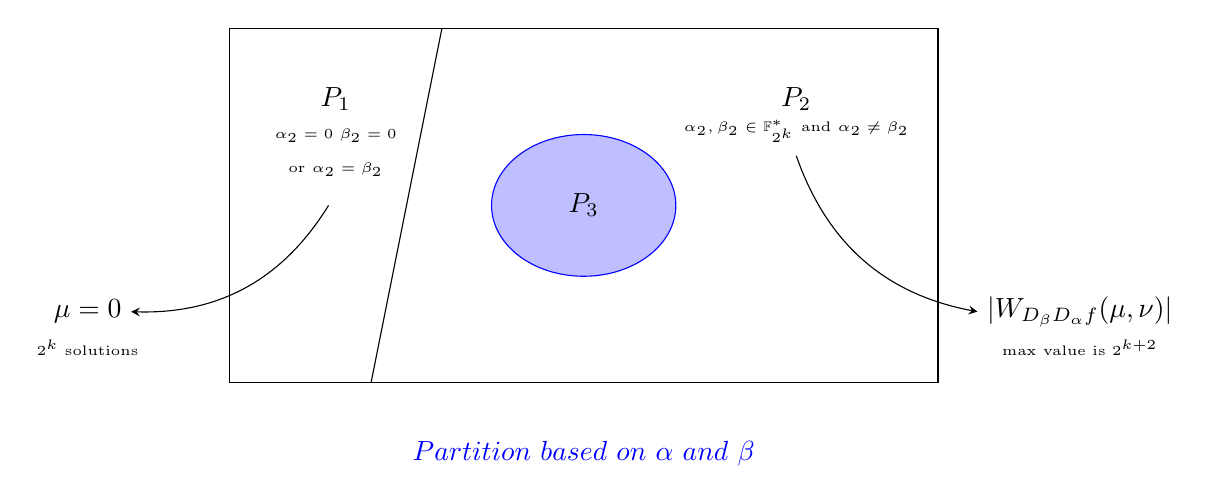
\begin{tikzpicture}[node distance=0.8cm, scale=0.9]
                    \def\evA{(2,0) -- (3,5)}
                    \def\evB{(5,2.5) ellipse (1.3cm and 1cm)}
                    \draw (0,0) -- (0,5) -- (10,5) -- (10,0) -- (0,0);
                    \draw[color=blue, fill=blue!25] \evB;
                    \draw \evA;
                    \begin{scope}
                        \clip \evA;
                        \fill[fill=blue!25] \evB;
                    \end{scope}
                    \node (n1) at (5,-1) {\textcolor{blue}{$ Partition~based~on~\alpha~and~\beta$}};
                    \node (n2) at (1.5,4) {$P_1$};
                    \node (n4) at (1.5,3) {\tiny$\text{or~}\alpha_2=\beta_2$} node[below of=n2,label={\tiny$ \alpha_2=0~\beta_2=0 $}]{};
                    \node (n3) at (8,4) {$P_2$} node[below of=n3,
                    label={\tiny$ \alpha_2,\beta_2\in\Fks\text{~and~}\alpha_2\ne\beta_2$}]{ };
                    \node (q1) at (-2,1) {$ \mu=0 $} node[below of=q1,
                    label={\tiny$ 2^k\text{~solutions} $}]{};
                    \node (q2) at (12,1) {$ |W_{D_{\beta}D_{\alpha}f}(\mu,\nu)| $} node[below of=q2,
                    label={\tiny max value is $ 2^{k+2} $}]{};
                    \node (p3) at (5,2.5) {$ P_3 $};
                    % \node (p4) at (5,2.5) {$ P_3 $};
                    % \node (q2) at (4,2) {$F\cap H^c$} node[below of=q2,
                    % label={\tiny$P(F\cap H^c)=0.004$}]{};
                    \path[->,>=stealth] (1.4,2.5) edge[bend left] node [right] {}
                    (q1.east);
                    \path[->,>=stealth] (8,3.2) edge[bend right] node [left] {}
                    (q2.west);
                \end{tikzpicture}
            \end{center}
    \end{frame}
    
    \begin{frame}
        \frametitle{The solutions of the equation}
    
        \begin{itemize}
            \item If $ S=\{0,\alpha_2,\beta_2,\alpha_2+\beta_2,y_0,y_0+\alpha_2,y_0+\beta_2,y_0+\alpha_2+\beta_2\} $, 
            we have 
            \begin{align*}
                &W_{D_{\beta}D_{\alpha}f}(\mu,\nu)\\
                =&\begin{cases}
                    2^{k+3}\cdot(-1)^{f_0^{**}},\text{if}~\tr\left(\mu\alpha_1+\nu\alpha_2\right)=0,\tr\left(\mu\beta_1+\nu\beta_2\right)=0 ~\text{and}~f_0^{**}+f_1^{**}=0\\
                    0,~\text{otherwise.}
                \end{cases}
            \end{align*}
            where $ f_0^{**} +f_1^{**} =\tr\left(\frac{\lambda\alpha_1}{\alpha_2}+\frac{\lambda\beta_1}{\beta_2}+\frac{\lambda(\alpha_1+\beta_1)}{\alpha_2+\beta_2}+\frac{\lambda\alpha_1}{y+\alpha_2}+\frac{\lambda\beta_1}{y+\beta_2}+\frac{\lambda(\alpha_1+\beta_1)}{y+\alpha_2+\beta_2}+\nu y\right) $ and 
            $ y\in\{y_0,y_0+\alpha_2,y_0+\beta_2,y_0+\alpha_2+\beta_2\} $. 

            % Thus we conclude $ \max_{\mu,\nu}|W_{D_{\beta}D_{\alpha}f}(\mu,\nu)|= 2^{k+3} $
        \end{itemize}
    \end{frame}

    \begin{frame}
        \frametitle{the solutions of }
    
        We need to prove two things: 
        \begin{itemize}
            \item There exists $ \mu\in\Fk $ such that $ S $ has $ 8 $ elements, i.e. condition \eqref{condition:0_root_condition_1} and \eqref{condition:y_0_root_condition_2} are both true.
            \item And there exists $ \nu\in\Fk $ satisfying 
            \begin{empheq}[left=\empheqlbrace]{align}\label{eq:3trace_0N_ijk}
                &\tr\left(\mu\alpha_1+\nu\alpha_2\right)=0\nonumber\\
                &\tr\left(\mu\beta_1+\nu\beta_2\right)=0\\
                &f_0^{**}+f_1^{**}=0.\nonumber
            \end{empheq}
        \end{itemize}
    
    \end{frame}

    \begin{frame}
        \frametitle{the first condition}
    
        \begin{itemize}
            \item Since we will always find $ \mu =\frac{\lambda(\alpha_2^2+\beta_2^2+\alpha_2\beta_2)}{\alpha_2^2\beta_2+\alpha_2\beta_2^2}\in\Fks $ making condition \eqref{condition:0_root_condition_1} true, we take $ \mu $ into 
            condition \eqref{condition:y_0_root_condition_2} to get 
            \begin{empheq}[left=\empheqlbrace]{align*}\label{eq:2trace_0Kloosterman}
                \tr\left(\frac{1}{\gamma^2+\gamma+1}\right)=&0\tag{*}\\ 
                \tr\left(\frac{\gamma^2}{\gamma^2+\gamma+1}\right)=&0. 
            \end{empheq} 
            where $ \gamma=\frac{\beta_2}{\alpha_2}\in\Fk\setminus\F_4 $.
            \item According to Lemma \eqref{Lemma:SumInv00}, the number of $ \gamma=\frac{\beta_2}{\alpha_2} $ satisfying equations above is $ L $. 
        \end{itemize}
    
    \end{frame}

    \begin{frame}
        \frametitle{the second condition}
    
        \begin{itemize}
            \item According to Lemma \eqref{lemma:N_ijk_trace}, 
            there always exist $ \nu\in\Fk $ that equations \eqref{eq:3trace_0N_ijk} hold true, which means:
            \begin{itemize}
                \item[\ding{110}] There always exist $ (\mu,\nu) $ 
                s.t. $ \max_{\mu,\nu}|W_{D_{\beta}D_{\alpha}f}(\mu,\nu)|= 2^{k+3} $
                % \footnote{Equality is established if there are only four solutions.} 
                for all points $ \alpha=(\alpha_1,\alpha_2),\beta=(\beta_1,\beta_2)\in\Fk^2 $ such that $ \alpha_2,\beta_2\in\Fks $, 
                $ \alpha_2\ne\beta_2 $ and $ \gamma=\frac{\beta_2}{\alpha_2} $ satisfies equation \eqref{eq:2trace_0Kloosterman}.
                \item[\ding{110}] Therefore, we can always find $ (\mu,\nu) $ 
                s.t. $ \max_{\mu,\nu}|W_{D_{\beta}D_{\alpha}f}(\mu,\nu)|= 2^{k+2} $ with $ \alpha_2,\beta_2\in\Fks,\alpha_2\ne\beta_2 $ and $ \gamma=\frac{\beta_2}{\alpha_2} $ in other cases.
            \end{itemize}
        \end{itemize}
        
    \end{frame}

    \begin{frame}
        \frametitle{The partition of $ \alpha,\beta $}
        \begin{figure}
            \caption{The partition of $ \alpha,\beta $}
            \begin{center}
                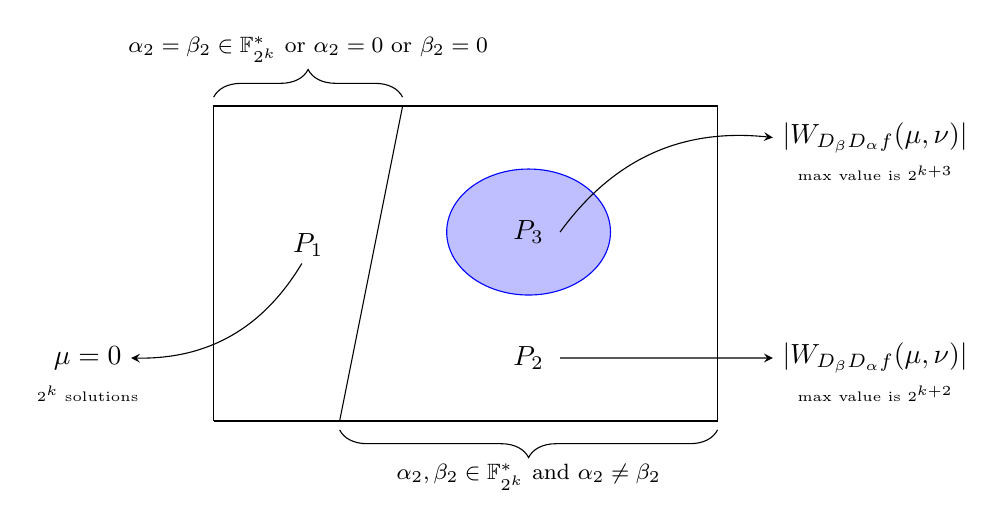
\begin{tikzpicture}[node distance=0.8cm, scale=0.8]
                    \def\evA{(2,0) -- (3,5)}
                    \def\evB{(5,3) ellipse (1.3cm and 1cm)}
                    \draw (0,0) -- (0,5) -- (8,5) -- (8,0) -- (0,0);
                    \draw[color=blue, fill=blue!25] \evB;
                    \draw \evA;
                    \begin{scope}
                        \clip \evA;
                        \fill[fill=blue!25] \evB;
                    \end{scope}
                    % \node (n1) at (5,-1) {\textcolor{blue}{$ Partition~based~on~\alpha~and~\beta$}};
                    \node (n2) at (1.5,2.8) {$P_1$};
                    % \node (n4) at (1.5,3) {\tiny$\text{or~}\alpha_2=\beta_2$} node[below of=n2,label={\tiny$ \alpha_2=0~\beta_2=0 $}]{};
                    \node (n3) at (5,1) {$P_2$};
                    %  node[below of=n3,label={\tiny$ \alpha_2,\beta_2\in\Fks\text{~and~}\alpha_2\ne\beta_2$}]{ };
                    \node (q1) at (-2,1) {$ \mu=0 $} node[below of=q1,
                    label={\tiny$ 2^k\text{~solutions} $}]{};
                    \node (q2) at (10.5,1) {$ |W_{D_{\beta}D_{\alpha}f}(\mu,\nu)| $} node[below of=q2,
                    label={\tiny max value is $ 2^{k+2} $}]{};
                    \node (p3) at (5,3) {$ P_3 $};
                    \node (p4) at (10.5,4.5) {$ |W_{D_{\beta}D_{\alpha}f}(\mu,\nu)| $} node[below of=p4,
                    label={\tiny max value is $ 2^{k+3} $}]{};
                    % \node (q2) at (4,2) {$F\cap H^c$} node[below of=q2,
                    % label={\tiny$P(F\cap H^c)=0.004$}]{};
                    \path[->,>=stealth] (1.4,2.5) edge[bend left] node [right] {}
                    (q1.east);
                    \path[->,>=stealth] (5.5,1) edge node [left] {}
                    (q2.west);
                    \path[->,>=stealth] (5.5,3) edge[bend left] node [left] {}
                    (p4.west);
                    \draw [decorate,decoration={brace,amplitude=10pt},xshift=0pt,yshift=4pt]
                    (0,5) -- (3,5) node [black,midway,yshift=0.6cm] 
                    {\footnotesize $ \alpha_2=\beta_2\in\Fks\text{~or~}\alpha_2=0~\text{or~}\beta_2=0$};
                    \draw [decorate,decoration={brace,mirror,amplitude=10pt},xshift=0pt,yshift=-4pt]
                    (2,0) -- (8,0) node [black,midway,yshift=-0.6cm] 
                    {\footnotesize $ \alpha_2,\beta_2\in\Fks\text{~and~}\alpha_2\ne\beta_2 $};
                \end{tikzpicture}
            \end{center}
        \end{figure}
    \end{frame}

    \begin{frame}
        \frametitle{Conclusion}
    
        For every points $ \alpha=(\alpha_1,\alpha_2)\in\Fk\times\Fks $, there exist $ L $ different $ \beta_2 $ 
        contributing to $ |W_{D_{\beta}D_{\alpha}f}(\mu,\nu)| = 2^{k+3} $, $ 2^k-2-L $ different $ \beta_2 $ leading 
        to  $ |W_{D_{\beta}D_{\alpha}f}(\mu,\nu)| = 2^{k+2} $, while $ \beta_1 $ can be any element of $ \Fk $. 

        Thus, for all points $ \alpha=(\alpha_1,\alpha_2),\beta=(\beta_1,\beta_2)\in\Fk\times\Fks $ with $ \alpha_2\ne\beta_2 $, 

    
    \end{frame}


    \begin{frame}
        \frametitle{Lemma}
%        \begin{lemma}
%            Let $ f $ be any $ n $-variable Boolean function and $ r $ be a positive integer smaller than $ n $. 
%            Then we have 
%            \[nl_r(f)\ge 2^{n-1}-\frac{1}{2}\sqrt{2^{2n}-2\sum_{a\in\Fn}nl_{r-1}(D_af)}.\]
%            where $ D_af(x) = f(x) + f(x+a) $ is the derivative of $ f $ at point $ a $.
%        \end{lemma}
%        
%        begin{lemma}\label{Lemma:SumInv00}
%            Let $n\geq 3$ be an arbitrary integer. We define
%            $$L=\#\left\{c\in\F_{2^n} : \mathrm{Tr}_1^n\left(\frac{1}{c^2+c+1}\right)=\mathrm{Tr}_1^n\left(\frac{c^2}{c^2+c+1}\right)=0\right\}.$$
%            Then we have $ L=2^{n-2}+\frac{3}{4}(-1)^n\widehat{I_1}(1)+\frac{1}{2}\left(1-(-1)^n\right) $, where $ \widehat{I_1}(1)=1-\sum_{t=0}^{\lfloor n/2\rfloor}(-1)^{n-t}\frac{n}{n-t}{{n-t}\choose {t}}2^t $.
%            % where $\widehat{I_1}(1)$ can be computed using Lemma~\ref{L:Kloostermansumsone}.
%        \end{lemma}
    \end{frame}
        
    \begin{frame}
        \frametitle{Lemma}
        
        \begin{lemma}\label{lemma:N_ij_trace}
            Assume  $ k\ge 2 $, let $ N_{i,j} =\left\lvert\left\{x\in\F_{2^k}\middle|\tr\left(\theta_1x+\gamma_1\right)=i,\tr\left(\theta_2x+\gamma_2\right)=j\right\}\right\rvert $ 
            where  $ \gamma_1,\gamma_2\in\F_{2^k} $ and $ \theta_1,\theta_2\in\F_{2^k}^* $ are distinct, then $ N_{0,0} =2^{k-2} $.
        \end{lemma}   
           
        \begin{proof}
            We have $ N_{0,0}+N_{0,1}+N_{1,0}+N_{1,1}=2^k $ and $ N_{0,0}+N_{0,1}=2^{k-1} $, $ N_{1,1}+N_{0,1}=2^{k-1}  $, then we get 
            $ N_{0,0} = N_{1,1} $. 
            Besides, $ N_{0,0}+N_{1,1} = \left\lvert\left\{x\in\F_{2^k}\middle|\tr\left((\theta_1+\theta_2)x+(\gamma_1+\gamma_2)\right)=0\right\}\right\rvert=2^{k-1} $  since $ \theta_1\ne \theta_2 $. 
            Therefore $ N_{0,0}=2^{k-2} $.
        \end{proof}
    \end{frame}
        % Thus $ nl_3(f) $ is bounded by the values of $ nl(D_bD_af) $.

        \begin{frame}
            \frametitle{Lemma}
        
            \begin{lemma}\label{lemma:N_ijk_trace}
                Assume  $ k\ge 3 $, let $ N_{i_1,i_2,i_3}=\left\lvert\left\{x\in\F_{2^k}\middle| \tr\left(\theta_1x+\gamma_1\right)=i_1,\tr\left(\theta_2x+\gamma_2\right)=i_2,\tr\left(\theta_3x+\gamma_3\right)=i_3 \right\} \right\rvert$, 
              where  $ \gamma_1,\gamma_2,\gamma_3\in\F_{2^k} $ and $ \theta_1,\theta_2,\theta_3\in\F_{2^k}^* $ are distinct and satisfy 
              $ \theta_3\ne\theta_1+\theta_2 $. Then $ N_{0,0,0}= 2^{k-3} $.
          \end{lemma}
        \end{frame}
        
        
        \begin{frame}
            \frametitle{Proof of Lemma 3}
          
            \begin{proof}
              The equations 
                \begin{equation}\label{eq:from_lemma_1}\left\{\begin{alignedat}{3}
                  &N_{0,0,0}+N_{0,0,1}=2^{k-2}\\
                  &N_{0,0,0}+N_{0,1,0}=2^{k-2}\\
                  &N_{0,0,0}+N_{1,0,0}=2^{k-2}.\\
                \end{alignedat}\right.\end{equation}
                will lead to $ N_{0,0,1}=N_{0,1,0}=N_{1,0,0} $. With the same reason we also obtain  $ N_{0,1,1}=N_{1,0,1}=N_{1,1,0} $. 
    
                Because $ \theta_1+\theta_2+\theta_3\ne 0 $, we can get equations: 
                \begin{align}\label{eq:sum_three_trace} 
                    &N_{1,0,1}+N_{1,1,0}+N_{0,1,1}+N_{0,0,0}\nonumber\\
                    =&\left\lvert\left\{x\in\F_{2^k}\middle|\tr\left(\left(\theta_1+\theta_2+\theta_3\right)x+\left(\gamma_1+\gamma_2+\gamma_3\right)\right)=0\right\}\right\rvert\\
                    =&2^{k-1}.\nonumber
                \end{align}
            \end{proof}
        \end{frame}   
        \begin{frame}
            \frametitle{Proof of Lemma 3}        
        
            \begin{proof}
                
            Combine $ N_{0,0,1}=N_{0,1,0}=N_{1,0,0} $,  $ N_{0,1,1}=N_{1,0,1}=N_{1,1,0} $, equations \eqref{eq:sum_three_trace} with equations $ N_{0,0,0}+N_{0,0,1}+N_{0,1,0}+N_{0,1,1}=2^{k-1} $, 
            % \begin{equation}\label{eq:sum_N_0jk}\left\{\begin{alignedat}{2}
            %     N_{0,0,0}+N_{0,0,1}+N_{0,1,0}+N_{0,1,1}=\left\lvert\left\{x\in\F_{2^k}\middle|\tr\left(\theta_1x+\gamma_1\right)=0\right\}\right\rvert=2^{k-1}\\
            %     N_{1,0,0}+N_{1,0,1}+N_{1,1,0}+N_{1,1,1}=\left\lvert\left\{x\in\F_{2^k}\middle|\tr\left(\theta_1x+\gamma_1\right)=1\right\}\right\rvert=2^{k-1}.\\
            % \end{alignedat}\right.\end{equation}
              we obtain the result $ N_{0,0,1}=N_{0,1,1} $. 
              Therefore from equations \eqref{eq:from_lemma_1} and equations \eqref{eq:sum_three_trace} we have 
              \begin{equation}\left\{\begin{alignedat}{2}
                      &N_{0,0,0}+N_{0,0,1}=2^{k-2}\\
                      &N_{0,0,0}+3N_{0,0,1}=2^{k-1}.
              \end{alignedat}\right.\end{equation}
              and the solution is $ N_{0,0,0}=N_{0,0,1}=2^{k-3} $.
            \end{proof}
        \end{frame}
    \makebottom     % 创建尾页  % 非标准命令

\end{document}